
\documentclass[12pt, a4paper]{article}
\usepackage[english]{babel}
\usepackage[utf8]{inputenc}
\usepackage{amsmath}
\usepackage{graphicx}


\title{\textbf{Genomic Computing Evaluation}\\Assignment 1: The Genome Browser}
\author{Fabrizio Frasca}
\date{\today}

\begin{document}
	
\maketitle
\clearpage

\section{UCSC Genome Browser}

\subsection*{(a)}

\textbf{Go to the genomic region chr6:45,296,054-45,518,819 of the Human assembly GRCh37/h19.}%

\textbf{\\ Which genes do you see in this region? On which strand are they?}%
\paragraph{} This region of human DNA contains part of the \textbf{SUPT3H} gene and part of the \textbf{RUNX2} gene. The former is present in 4 variants and the latter is present in 3 variants in the UCSC database.%
\paragraph{} SUPT3H is on the \textbf{reverse strand} (arrows pointing towards left), whereas the RUNX2 is on the \textbf{forward strand} (arrows pointing towards right).	

\subsection*{(b)}

\textbf{Enable GC Percent [dense] from Mapping and Sequencing tracks and CpG Islands [show] from Regulation tracks.\\ Now zoom into the region chr6:45,330,000-45,400,000.}%

\textbf{\\ Does the GC composition reach a peak in correspondence of some important regulatory element?}%
\paragraph{}Yes, it does. In particular, as shown in figure \ref{GC peaks}, two significant peaks are observed: one corresponds to the promotorial region of the SUPT3H gene and the other one corresponds to the promotorial region of one of the variants of RUNX2 gene.

\begin{figure}[h]
		\centering
		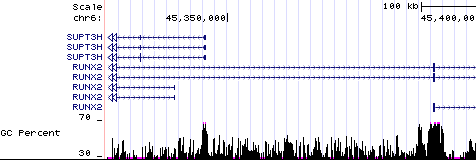
\includegraphics[width = .8\textwidth]{GC_peaks}
		\caption{Peaks for the GC signal}
		\label{GC peaks}
\end{figure}
	
\textbf{\\ In which region do you notice the most regulatory activity? Does it involve a CpG island? (If yes, report Coordinates, Chromosome band, Genomic size of the first (along the genome) of them)}%
\paragraph{}The regions interested by regulatory activities the most are the ones detected above: \textbf{chr6:45,343,511-45,348,384} ca. for the promotorial region of SUPT3H and \textbf{chr6:45,387,920-45,392,851} ca., corresponding to the promoter of one of the variants for the RUNX2 gene.

\begin{figure}[h]
	\centering
	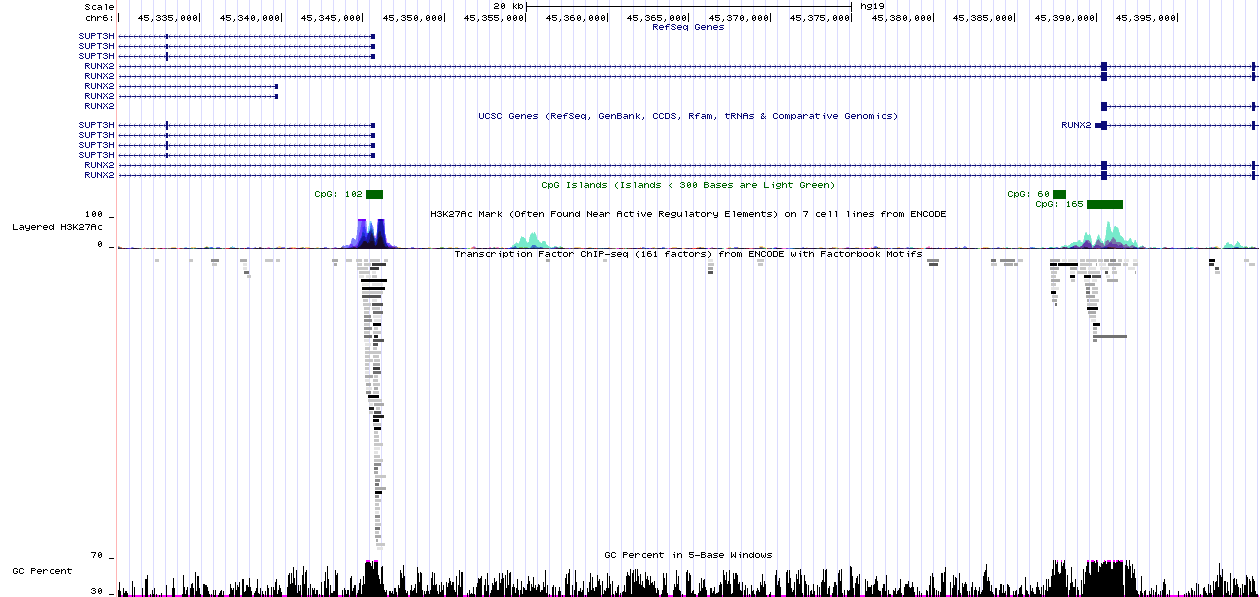
\includegraphics[width = \textwidth]{regulatory_regions}
	\caption{Regions involved in regulatory activities}
	\label{regulatory regions}
\end{figure}

\paragraph{}These regions are promisingly characterized by regulatory activities because of the conjugate presence of CpG islands, strong evidence of H3K27 acetylation and the binding of several transcription factors, as shown by the relative tracks in figure \ref{regulatory regions}.

\paragraph{}The first CpG island encountered by proceeding in the direction of the forward strand is the one corresponding to the promotorial region of the SUPT3H region. In particular, it has:%

\begin{align*}
&\textbf{coordinates: } &&\text{chr6:45345186-45346261}\\
&\textbf{chromosome band: } &&\text{6p21.1}\\
&\textbf{genomic size: } && 1076
\end{align*}

\begin{figure}[t]
	\centering
	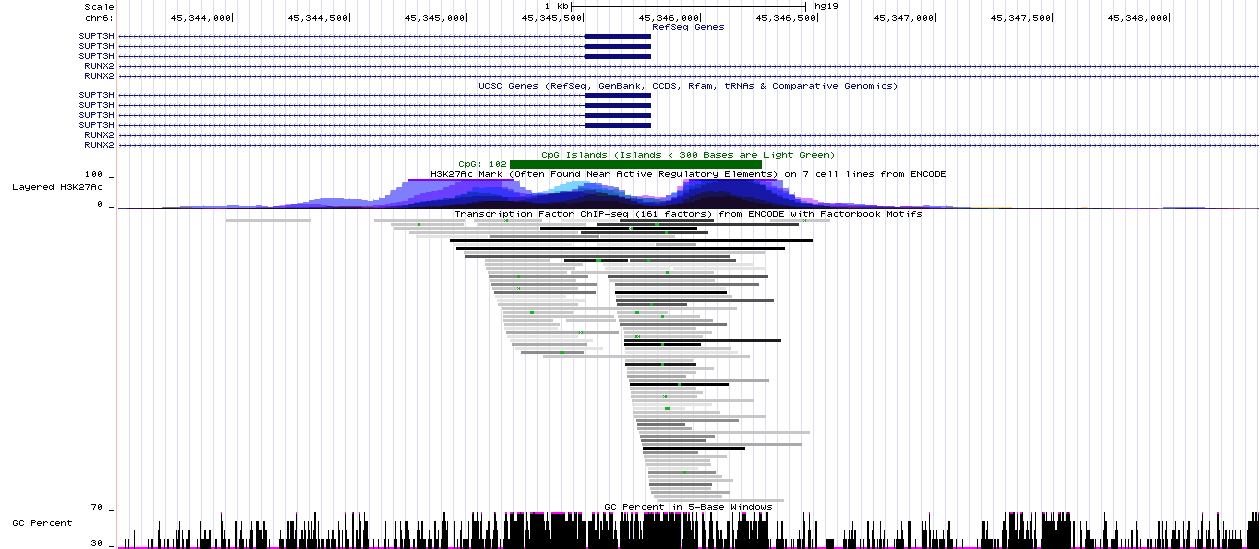
\includegraphics[width = \textwidth]{CpG_island}
	\caption{The first CpG island, along with other 'regulatory tracks' in the same region}
	\label{CpG island}
\end{figure}

\section{BLAT }

\textbf{Consider the following FASTA file:}

\begin{verbatim}
	> read1
	ACCACATATTTTGCAAATTTTGCATGCTGAAACTTCTCAACCAGAAGAAAGGGCCTTCACAG
	TGTCCTTTATGTAAGAATGATATAACCAAAAGGAGCCTACAAGAAAGTACGAGATTTAGTCAA
	CTTGTTGAAGAGCTA
	> read2
	ACCACATATTTTGCAAATTTTGCATGCTGATACTTCTCAACCAGAAGAAAGGGCCTTCACAGT
	GTCCTTTATGTAAGAATGATATAACCAAAAGGAGCCTACAAGAAAGTACGAGATTTAGTCAAC
	TTGTTGAAGAGCTA
	> read3
	ACCACATATTTTGCAAATTTTGCATGCTGATACTACTCAACCAGAAGAAAGGGCCTTCACAGT
	GTCCTTTATGTAAGAATGATATAACCAAAAGGAGCCTACAAGAAAGTACGAGATTTAGTCAAC
	TTGTTGAAGAGCTA
	> read4
	ACCACATATTTTGCAAATTTTGCATGCTGATACTACTCAACCAGAAGAAAGGGCCTTCACAGT
	GTCCTTTATGTAAGAATGATATAACCAAAAGGAGCCTAAAGAAAGTACGAGATTTAGTCAACT
	TGTTGAAGAGCTA
	> read5
	ACCACATATTTTGCAAATTTGCATGCTGAAACTTCTCAACCAGAAGAAAGGGCCTTCACAGTG
	TCCTTTATGTAAGAATGATATAACCAAAAGGAGCCTACAAGAAAGTACGAGATTTAGTCAACT
	TGTTGAAGAGCTA
	> read6
	ATGAATGTAGAAAAGGCTGAATTCTGTAATAAAAGCAAACAGCCTGGCTTAGCAAGGAGCCAA
	CATAACAGATGGGCTGGAAGTAAGGAAACATGTAATGATAGGCGGACTCCCAGCACAGAAAAA
	AAGGTAGATCTGAA
\end{verbatim}

\textbf{\\ Use BLAT to map these sequences onto Human assembly GRCh37/h19.}%

\textbf{\\Does each read map in a single region?}%

\paragraph{}No, it does not. For instance, read 1 maps on chr17:41256928-41258550 and chr4:146760838-146760862 regions at the same time, see figure \ref{BLAT results}.%

\begin{figure}[h]
	\centering
	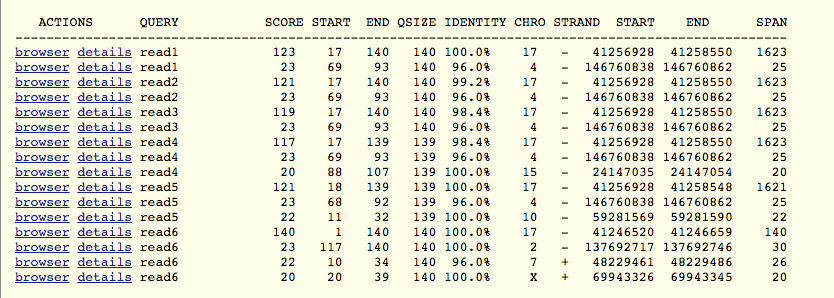
\includegraphics[width = \textwidth]{BLAT_results}
	\caption{Results for the alignment from BLAT}
	\label{BLAT results}
\end{figure}

\textbf{\\ On the base of the alignment score and sequence identity, which genome region do the reads belong?}%

\paragraph{}It is fairly evident that all the alignments with high score map to the same genome region and they are characterized by very high identity as well. The region is \textbf{chr17:41256928-41258550} for all the reads 1-5 and \textbf{chr17:41246520-41246659} for read 6, which is definitely similar. Other alignments have pretty good identity, but they must be discarded since their score is poor.

\textbf{\\ Which gene this reads come from?}%
\paragraph{}By clicking on the “browser” link for one of the mapping with highest score, we can realize the interested gene is \textbf{BRCA1}.

\end{document}